%\documentclass[border = 3mm,
%               tikz]{standalone}
\documentclass{article}
\usepackage{tikz}
\usepackage{siunitx}
\usepackage{forest}
\usepackage{cleveref}
\usetikzlibrary{arrows.meta,shapes,positioning}
\usepackage{../themeKonstanz}
\usepackage{pgfplots}

\usetikzlibrary{arrows,shapes,positioning}
\usetikzlibrary{decorations.markings}

\tikzset{fontscale/.style = {font=\relsize{#1}}
    }
\usetikzlibrary{arrows.meta,shapes,positioning}
\tikzset{MyArrow/.style={single arrow, draw, minimum width=8mm, minimum height=5mm,
                         inner sep=0mm, single arrow head extend=1mm}}

\begin{document}

\begin{figure}
\centering
    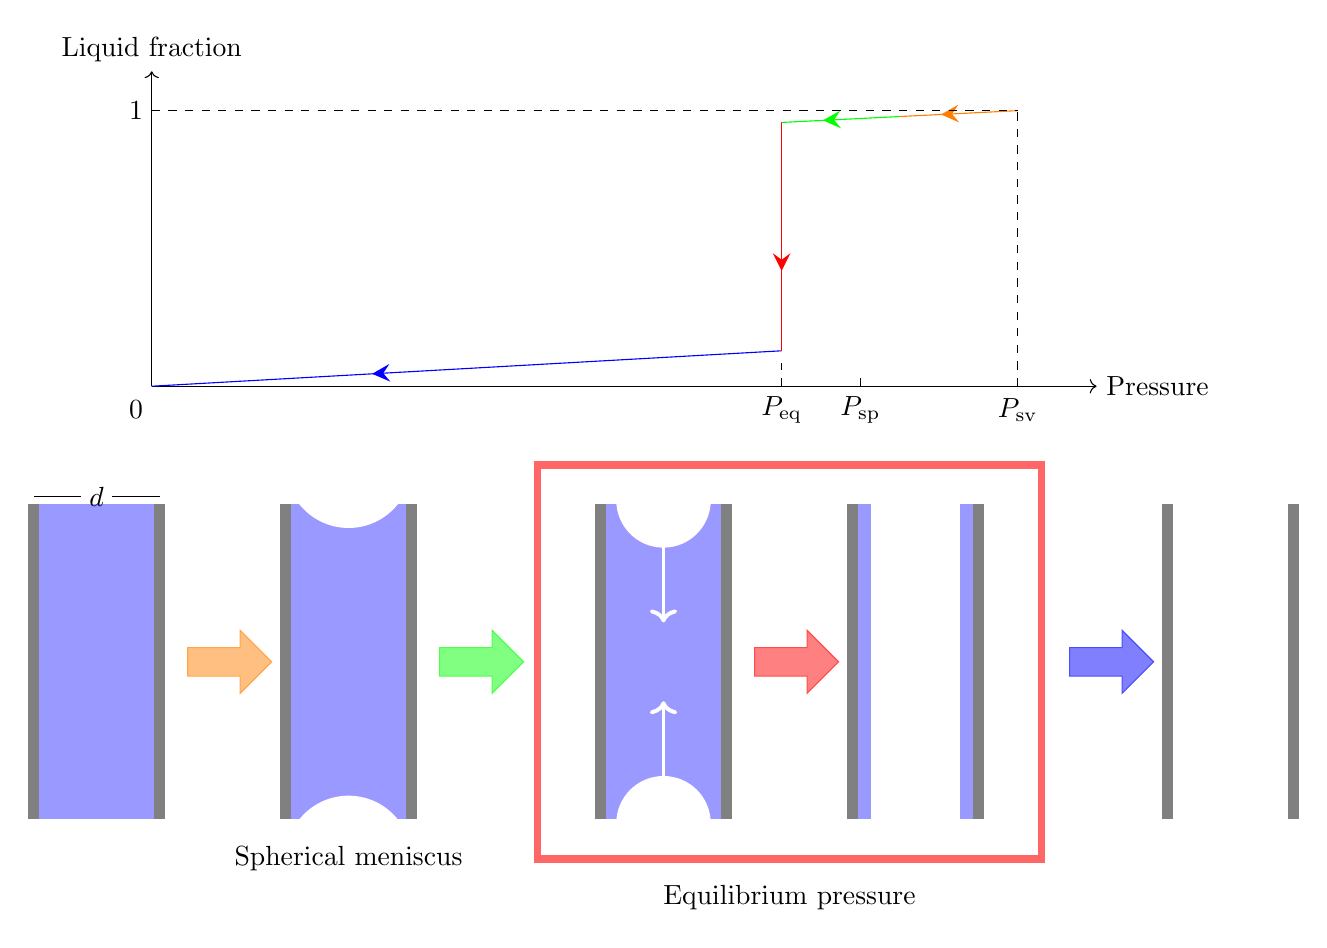
\begin{tikzpicture}[pore/.style = {line width = 0.15cm, color = gray},
                        film/.style = {line width = 0.18cm, color = blue!40},
                        thick_film/.style = {line width = 0.3cm, color = blue!40},
                        graph_label/.style={color = gray, line width = 0.05cm},
                        pore_collapse/.style = {color = blue!50, line width = 0.07cm, ->},
                        MyArrow/.style={single arrow, draw, minimum width=8mm, minimum height=5mm,
                         inner sep=0mm, single arrow head extend=1mm}]
        \pgfdeclarelayer{bg}    % declare background layer
        \pgfdeclarelayer{bbg}    % declare backbackground layer
        \pgfsetlayers{bbg,bg,main}  % set the order of the layers (main is the standard layer)
        \tikzstyle arrowstyle=[scale=2]
        \tikzstyle directed=[postaction={decorate,decoration={markings,
            mark=at position .65 with {\arrow[arrowstyle]{stealth}}}}]
        \begin{scope}
            \foreach \Xcoor in {0, 1.6, 3.2, 4.8, 7.2, 8.8, 10.4, 12, 14.4, 16}
            \draw[pore] (\Xcoor,0) -- (\Xcoor,4);
            \draw (0.6,4.1) -- (0,4.1); 
            \draw (1,4.1) -- (1.6,4.1); 
            \node at (0.8,4.1) {$d$};
            \node[draw = orange!70, fill = orange!50, MyArrow] at (2.4, 2) {\phantom{arrow}};
            \node[draw = green!70, fill = green!50, MyArrow] at (5.6, 2) {\phantom{arrow}};
            \node[draw = red!70, fill = red!50, MyArrow] at (9.6, 2) {\phantom{arrow}};
            \node[draw = blue!70, fill = blue!50, MyArrow] at (13.6, 2) {\phantom{arrow}};
            %
            \draw[color = red!60, line width = 0.1cm] (6.4,-0.5) -- (12.8,-0.5) -- (12.8,4.5) -- (6.4,4.5) -- cycle; 
            \node at (9.6,-1) {Equilibrium pressure};
            \node at (4,-0.5) {Spherical meniscus};
            \begin{pgfonlayer}{bg}    % select the background layer
                %full pore
                \fill[blue!40] (0,0) -- (0,4)  -- (1.6,4) -- (1.6,0) -- cycle ;
                %full pore with menisci
                \fill[blue!40] (3.2,0) -- (3.2,4)  -- (4.8,4) -- (4.8,0) -- cycle ;
                \path [draw = none, fill = white](3.2,4.5) arc[start angle = -180, end angle = 0, radius=0.8];
                \path [draw = none, fill = white](3.2,-0.5) arc[start angle = 180, end angle = 0, radius=0.8];
                %emptying pore
                \fill[blue!40] (7.2,0) -- (7.2,4)  -- (8.8,4) -- (8.8,0) -- cycle ;
                \path [draw = none, fill = white](7.4,4.05) arc[start angle = -180, end angle = 0, radius=0.6];
                \path [draw = none, fill = white](7.4,-0.05) arc[start angle = 180, end angle = 0, radius=0.6];
                \draw[color = white, ->, line width = 0.5mm] (8,0) -- (8,1.5);
                \draw[color = white, ->, line width = 0.5mm] (8,4) -- (8,2.5);
                %filmed pore
                \draw[film] (10.55,0) -- (10.55,4);
                \draw[film] (11.85,0) -- (11.85,4);
            \end{pgfonlayer}
        \end{scope}
        \begin{scope}[xshift = 1.5cm, yshift=5.5cm]
            \draw[->] (0,0) -- (0,4) node[anchor=south] {Liquid fraction};
            \draw[->] (0,0) -- (12,0) node[anchor=west] {Pressure};
            %blue
            \draw[color = blue, directed] (8,0.45) -- (0,0);
            %red
            \draw[color = red, directed] (8,3.35) -- (8,0.45);
            %green
            \draw[color = green, directed] (9.5,3.425) -- (8,3.35);
            %orange
            \draw[color = orange, directed] (11,3.5) -- (9.5,3.425);
            %DASHED
            \draw[dashed] (0,3.5) -- (11,3.5);  %1
            \draw[dashed] (11,0) -- (11,3.5);  %psat
            \draw[dashed] (8,0) -- (8,0.3);  %peq
            \draw[dashed] (9,0) -- (9,0.15);  %psp
            %labels
            \node at (-0.2,-0.3) {$0$};
            \node at (-0.2,3.5) {$1$};
            \node at (11,-0.3) {$P_\mathrm{sv}$};
            \node at (8,-0.3) {$P_\mathrm{eq}$};
            \node at (9,-0.3) {$P_\mathrm{sp}$};
        \end{scope}
    \end{tikzpicture}
    \caption{Desorption isotherm of a straight cylindrical pore. Below, the processes inside the pore are illustrated. The colors of the broad arrow's colors correspond to the pressure ranges of the isotherm in the same color. Significant is the desorption at equilibirum pressure.}
    \label{fig:perf-cyl-pore-evap}
\end{figure}
\end{document}